We recall that our goal is to compute the expectation in \eqref{BS_formula_rbergomi}. In fact, as seen in Section \ref{sec:Simulation of the rBergomi model}, we need   $2N$-dimensional Gaussian inputs for the used  hybrid  scheme ($N$ is the number of time steps in  the time grid), namely
\begin{itemize}
	\item $\mathbf{W}^{(1)}=\{W^{(1)}_i\}_{i=1}^N$: The $N$ Gaussian random variables that are defined in Section  \ref{sec:The rBergomi model}.
	\item $\mathbf{W}^{(2)}=\{W^{(2)}_j\}_{j=1}^N$: An artificially introduced $N$ Gaussian random variables that are used for left-rule points in the hybrid scheme, as explained in Section  \ref{sec:Simulation of the rBergomi model}.
\end{itemize}
We can rewrite \eqref{BS_formula_rbergomi} as 
\begin{align}\label{BS_formula_rbergomi_2}
C_{\text{RB}}\left( T, K \right)&=\text{E}\left[C_{\text{BS}}\left( S_0 = \operatorname{exp}\left(\rho \int_0^T \sqrt{v_t} dW_t^1 - \frac{1}{2}
\rho^2 \int_0^T v_t dt\right),\ k = K, \ \sigma^2 = (1-\rho^2)
\int_0^T v_t dt \right) \right] \nonumber \\
&\approx \int_{\rset^{2N}} C_{BS} \left(G(\mathbf{W}^{(1)},\mathbf{W}^{(2)})\right) \rho_{N}(\mathbf{W}^{(1)})  \rho_{N}(\mathbf{W}^{(2)}) d\mathbf{W}^{(1)} d\mathbf{W}^{(2)} \nonumber \\
&:=C_{RB}^{N},
\end{align}
where $G$  maps  $2N$ independent standard Gaussian random inputs to the parameters fed to Black-Scholes formula, and  $\rho_N$ is the multivariate Gaussian density, given by 
\begin{equation*}\label{eq: multivariate gaussian distribution}
\rho_N(\mathbf{z})=\frac{1}{(2 \pi)^{N/2}} e^{-\frac{1}{2} \mathbf{z}^T \mathbf{z}} \PERIOD
\end{equation*} 
Therefore, the initial integration problem that we are solving lives in $2N$-dimensional space, which becomes very large as the number of time steps $N$, used in the hybrid scheme, increases.

Our approach of approximating the expectation in \eqref{BS_formula_rbergomi_2} is based on  hierarchical adaptive sparse grids, using the same construction as in MISC, proposed in \cite{haji2016multi}. We describe the  MISC method in our context in Section \ref{sec:Details of the MISC}.  To make an effective use of MISC, we  first apply two transformations to overcome the issue of facing a high dimensional integrand due to the discretization scheme used for simulating the rBergomi dynamics. The first transformation consists of applying a hierarchical  path generation method, based on Brownian bridge (Bb) construction, with the aim of reducing the effective dimension as  described  in Section \ref{sec:Brwonian bridge construction}. The second transformation consists of applying Richardson extrapolation to reduce the bias, resulting in reducing  the maximum number of dimensions needed for the integration problem. Details about  Richardson extrapolation  are provided in Section \ref{sec:Richardson extrapolation}.

If we denote by $\mathcal{E}_{\text{tot}}$ the total error of approximating the  expectation in \eqref{BS_formula_rbergomi} using the MISC estimator, $Q_N$, then we have a natural error decomposition
\red{
\begin{align}\label{eq:total_error}
\mathcal{E}_{\text{tot}} & \le \abs{C_{\text{RB}}-C_{\text{RB}}^N}+\abs{C_{\text{RB}}^N-Q_{N}} \le \mathcal{E}_B(N)+ \mathcal{E}_Q(\text{TOL}_{\text{MISC}},N),
\end{align}}
where  $\mathcal{E}_Q$ is the quadrature error, $\mathcal{E}_B$  is the bias, and $C_{\text{RB}}^N$ is the biased price computed with $N$ time steps as given by \eqref{BS_formula_rbergomi_2}.

\subsection{The MISC method}\label{sec:Details of the MISC}

We assume that we want to approximate the expected value $\text{E}[f(Y)]$ of an analytic function $f\colon \Gamma \to \rset$ using a tensorization of quadrature formulas over $\Gamma$.

To introduce simplified notations, we start with the one-dimensional case. Let us denote by $\beta$ a non-negative integer, referred to as a ``stochastic discretization level", and by $m: \nset \rightarrow \nset$  a strictly increasing function with $m(0)=0$ and $m(1)=1$, that we call  ``level-to-nodes function". At level $\beta$, we consider a set of $m(\beta)$ distinct quadrature points in $\rset$, $\mathcal{H}^{m(\beta)}=\{y^1_\beta,y^2_\beta,\dots,y_\beta^{m(\beta)}\} \subset \rset$, and a set of quadrature weights, $\boldsymbol{\omega}^{m(\beta)}=\{\omega^1_\beta,\omega^2_\beta,\dots,\omega_\beta^{m(\beta)}\}$. We also let $C^0(\rset)$ be the set of real-valued continuous functions over $\rset$. We then define the quadrature operator as
\begin{equation*}
Q^{m(\beta)}:C^0(\rset) \rightarrow \rset, \quad Q^{m(\beta)}[f]= \sum_{j=1}^{m(\beta)} f(y^j_\beta) \omega_\beta^j.
\end{equation*}
\red{In our case, we have in \eqref{BS_formula_rbergomi_2} a multi-variate integration problem with,  $f=C_{\text{BS}}\circ G$, $\mathbf{Y}=(\mathbf{W}^{(1)},\mathbf{W}^{(2)})$, and  $\Gamma=\rset^{2N}$, in the previous notations. Furthermore, since we are dealing with Gaussian densities, using Gauss-Hermite quadrature points is the appropriate choice}.

We define for any multi-index $\boldsymbol{\beta} \in \nset^{2N}$
$$Q^{m(\boldsymbol{\beta})}: C^0(\rset^{2N}) \rightarrow \rset,\quad  Q^{m(\boldsymbol{\beta})}= \bigotimes_{n = 1}^{2N} Q^{m(\beta_n)} \COMMA $$
where the $n$-th quadrature operator is understood to act only on the $n$-th variable of $f$. Practically, we obtain the value of $Q^{m(\boldsymbol{\beta})}[f]$  by using the grid $\mathcal{T}^{m(\boldsymbol{\beta})}= \prod_{n = 1}^{2N}  \mathcal{H}^{m(\beta_n)}$, with cardinality $\#\mathcal{T}^{m(\boldsymbol{\beta})}=\prod_{n=1}^{2N} m (\beta_n)$, and computing
$$ Q^{m(\boldsymbol{\beta})}[f]= \sum_{j=1}^{\#\mathcal{T}^{m(\boldsymbol{\beta})}} f(\hat{y}_j) \bar{\omega}_j \COMMA$$
where $\hat{y}_j \in \mathcal{T}^{m(\boldsymbol{\beta})}$ and $\bar{\omega}_j$ are  products of weights of the univariate quadrature rules. To simplify notation, hereafter, we replace  $Q^{m(\boldsymbol{\beta})}$ by $Q^{\boldsymbol{\beta}}$.

A direct approximation $\expt{f[\mathbf{Y}]} \approx Q^{\boldsymbol{\beta}}[f]$ is not an appropriate option  due to the well-known ``curse of dimensionality". \red{We use  a hierarchical adaptive sparse grids quadrature strategy, specifically using the same
construction as MISC}, and which uses  stochastic discretizations  and a classic sparsification approach to obtain an effective approximation scheme for $\expt{f}$. 

To be concrete, in our setting, we are left with a $2N$-dimensional Gaussian random input, which is chosen independently, resulting in  $2N$ numerical parameters for MISC, which we use as the basis of the multi-index construction. For a multi-index $\boldsymbol{\beta} = (\beta_n)_{n=1}^{2N} \in \mathbb{N}^{2N}$, we denote  by
$Q_N^{\boldsymbol{\beta}}$,   the result of approximating \eqref{BS_formula_rbergomi_2} with a number of quadrature points  in the $i$-th dimension equal to  $m(\beta_i)$. We further define the set of
differences $\Delta Q_N^{\boldsymbol{\beta}}$ as follows: for a single index $1 \le i \le 2N$,
let
\begin{equation*}
\Delta_i Q_N^{\boldsymbol{\beta}} = \left\{ 
\aligned 
 Q_N^{\boldsymbol{\beta}} &- Q_N^{\boldsymbol{\beta}'}  \text{, with } \boldsymbol{\beta}' =\boldsymbol{\beta} - e_i, \text{ if } \boldsymbol{\beta}_i>0 \COMMA \\
 Q_N^{\boldsymbol{\beta}} &, \quad  \text{ otherwise,}
\endaligned
\right.
\end{equation*}
where $e_i$ denotes the $i$th $2N$-dimensional unit vector. Then, $\Delta
Q_N^{\boldsymbol{\beta}}$ is defined as
\begin{equation*}
\Delta Q_N^{\boldsymbol{\beta}} = \left( \prod_{i=1}^{2N} \Delta_i \right) Q_N^{\boldsymbol{\beta}}.
\end{equation*}
For instance, when $N = 1$, then 
\begin{multline*}
	\Delta Q_1^{\boldsymbol{\beta}} = \Delta_2 \Delta_1 Q_1^{(\beta_1, \beta_2)} = \Delta_2\left( Q_1^{(\beta_1,
		\beta_2)} - Q_1^{(\beta_1-1,\beta_2)} \right) = \Delta_2 Q_1^{(\beta_1,
		\beta_2)} - \Delta_2 Q_1^{(\beta_1-1,\beta_2)} 
	\\= Q_1^{(\beta_1, \beta_2)} - Q_1^{(\beta_1, \beta_2-1)} - Q_1^{(\beta_1-1, \beta_2)} + Q_1^{(\beta_1-1, \beta_2-1)}.
\end{multline*}
Given the definition of $C_{RB}^{N}$ by \eqref{BS_formula_rbergomi_2}, we have the telescoping property
\begin{equation*}
C_{RB}^{N}=Q_N^\infty = \sum_{\beta_1=0}^\infty \cdots \sum_{\beta_{2N} = 0}^\infty \Delta
Q_N^{(\beta_1, \ldots, \beta_{2N})} = \sum_{\boldsymbol{\beta} \in \mathbb{N}^{2N}} \Delta Q_N^{\boldsymbol{\beta}}.
\end{equation*}
 The MISC estimator used for approximating \eqref{BS_formula_rbergomi_2}, and using a set of multi-indices $\mathcal{I}\subset \nset^{2N}$ is given by
\begin{equation}\label{eq:MISC_quad_estimator}
	Q_N^{\mathcal{I}} = \sum_{\boldsymbol{\beta} \in \mathcal{I}} \Delta Q_N^{\boldsymbol{\beta}}.
\end{equation}
The quadrature error in this  case  is given by
\begin{equation}\label{eq:quadrature error}
	\mathcal{E}_Q(\text{TOL}_{\text{MISC}},N) =\abs{Q_N^\infty - Q_N^\mathcal{I}} \le \sum_{\boldsymbol{\beta} \in \mathbb{N}^{2N} \setminus
		\mathcal{I}} \abs{\Delta Q_N^{\boldsymbol{\beta}}}.
\end{equation}
We define the work contribution, $\Delta \mathcal{W}_{\boldsymbol{\beta}}$, to be the computational cost  required to add  $\Delta Q_N^{\boldsymbol{\beta}}$ to $Q^{\mathcal{I}}_N$, and the error contribution, $\Delta E_{\boldsymbol{\beta}}$, to be  a measure of how much the quadrature error, defined in \eqref{eq:quadrature error}, would decrease once $\Delta Q_N^{\boldsymbol{\beta}}$  has been added to  $Q^{\mathcal{I}}_N$, that is 
\begin{align}\label{eq:Work_error_contributions}
\Delta \mathcal{W}_{\boldsymbol{\beta}} &= \text{Work}[Q^{\mathcal{I} \cup \{\boldsymbol{\beta}\}}_N]-\text{Work}[Q^{\mathcal{I}}_N] \nonumber\\
\Delta E_{\boldsymbol{\beta}} &= \abs{Q^{\mathcal{I} \cup \{\boldsymbol{\beta}\}}_N-Q^{\mathcal{I}}_N}.
\end{align}
 The  construction of the optimal  $\mathcal{I}$ will be done by profit thresholding, that is, for a certain threshold value $\bar{T}$, and a profit of a hierarchical surplus defined by
 \begin{equation*}
 P_{\boldsymbol{\beta}}= \frac{\abs{\Delta E_{\boldsymbol{\beta}}}}{\Delta\mathcal{W}_{\boldsymbol{\beta}}},
 \end{equation*}
  where the optimal index set  $\mathcal{I}$  for MISC  is given by 
 $\mathcal{I}=\{\boldsymbol{\beta}: P_{\boldsymbol{\beta}}	 \ge \bar{T}\}$.
\red{\begin{remark}
The analiticity assumption, stated in the beginning of Section \ref{sec:Details of the MISC}, is crucial for the optimal performance of our proposed method. In fact, although we face the issue of the  ``curse of dimensionality" when increasing $N$, the analiticity of $f$ implies an exponential convergence for sparse grids quadrature.
\end{remark}} 
\begin{remark}
	The choice of the hierarchy of quadrature points, $m(\boldsymbol{\beta})$, is flexible in the MISC algorithm and can be fixed by the user, depending on the convergence properties of the problem at hand. For instance, for the sake of reproducibility, in our numerical experiments we used a linear hierarchy: $m(\beta)=4 (\beta-1)+1,\: 1 \le \beta $, for results of parameter set $1$ in Table \ref{table:Reference solution, using MC with $500$ time steps, of Call option price under rBergomi model, for different parameter constellation.}. For the remaining parameter sets in Table  \ref{table:Reference solution, using MC with $500$ time steps, of Call option price under rBergomi model, for different parameter constellation.}, we used a geometric hierarchy: $m(\beta)=2^{\beta-1}+1, \:1 \le \beta $.
\end{remark} 
\begin{remark}
As emphasized in \cite{haji2016multi}, one important requirement to get the optimal performance of the MISC method is to check  the error convergence, defined by \eqref{eq:Work_error_contributions},  of first and mixed difference operators. We checked this requirement in all our numerical experiments, and for illustration, we show in Figures  \ref{fig:first_diff_comp_K_1_H_002} and \ref{fig:second_diff_comp_K_1_H_002}, the error convergence of first and second order differences for the case of parameter set $2$ in Table \ref{table:Reference solution, using MC with $500$ time steps, of Call option price under rBergomi model, for different parameter constellation.}.  These plots show that: i) $\Delta \text{E}_{\boldsymbol{\beta}}$ decreases exponentially fast with respect to $\beta_i$, and ii) $\Delta \text{E}_{\boldsymbol{\beta}}$ has a  product structure since  we  observe  a faster error decay for second differences compared to corresponding first difference operators.
\end{remark} 

\begin{figure}[h!]
	\centering
	\begin{subfigure}{.4\textwidth}
		\centering
		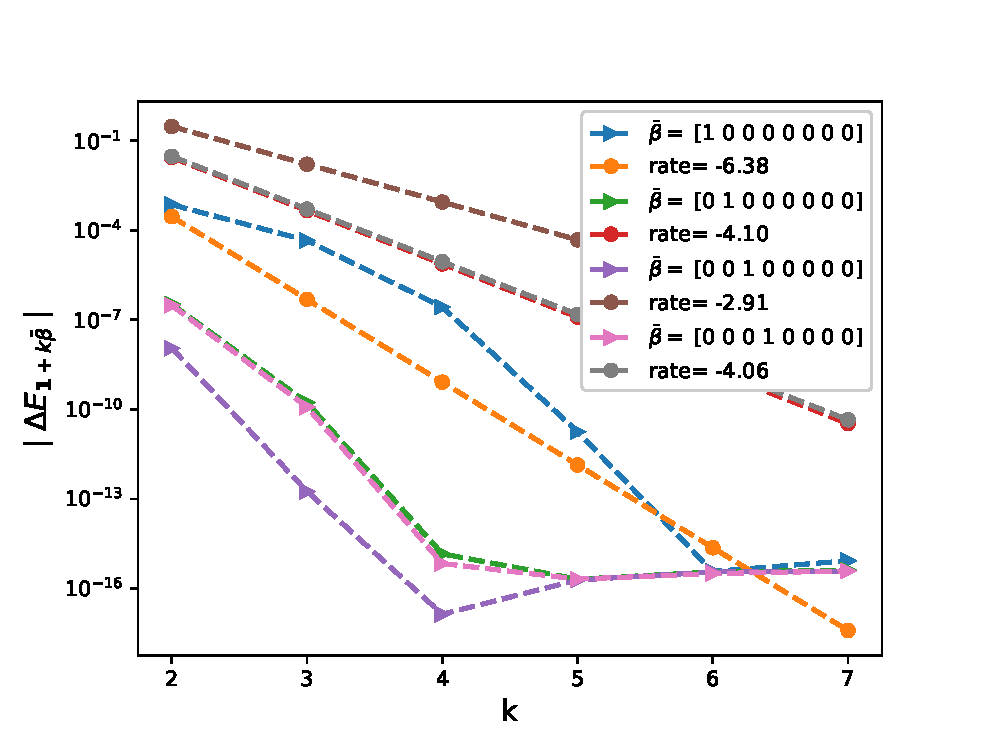
\includegraphics[width=1\linewidth]{./figures/rBergomi_mixed_error_rates/without_change_measure/N_4/H_002/first_difference_rbergomi_4steps_H_002_K_1_totally_hierarch_with_rate_W1}
		\caption{}
		\label{fig:sub3}
	\end{subfigure}%
	\begin{subfigure}{.4\textwidth}
		\centering
		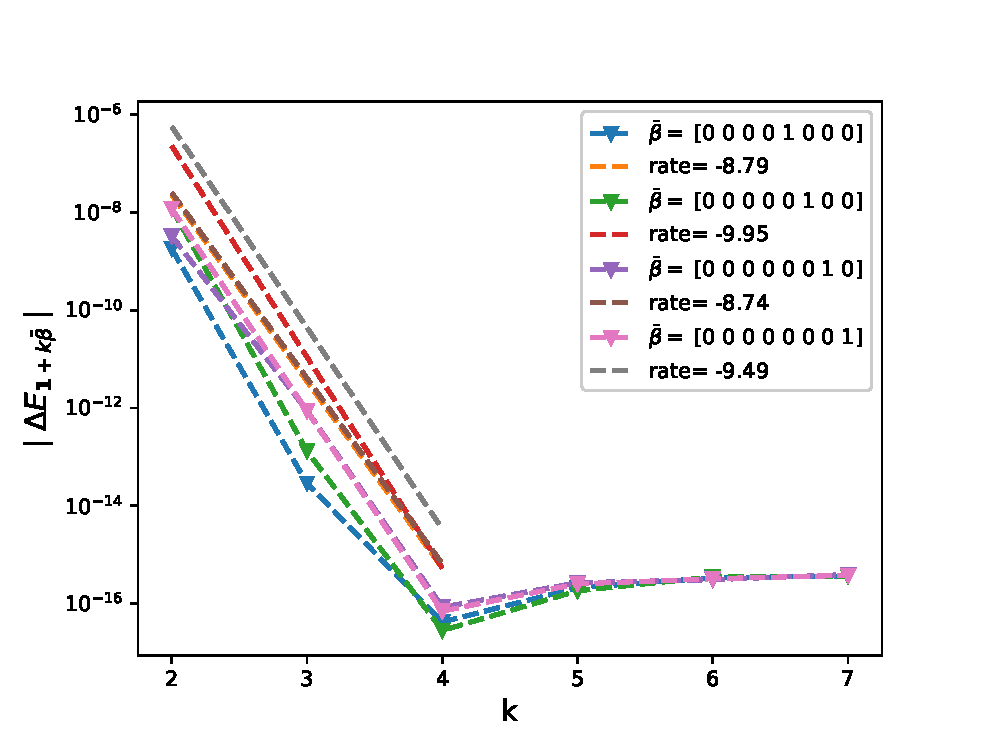
\includegraphics[width=1\linewidth]{./figures/rBergomi_mixed_error_rates/without_change_measure/N_4/H_002/first_difference_rbergomi_4steps_H_002_K_1_totally_hierarch_with_rate_W2}
		\caption{}
		\label{fig:sub4}
	\end{subfigure}
	
	
	
	\caption{The rate of error convergence of first order differences $\abs{\Delta \text{E}_{\boldsymbol{\beta}}}$, defined by \eqref{eq:Work_error_contributions}, ($\boldsymbol{\beta}=\mathbf{1}+k \bar{\boldsymbol{\beta}}$) with respect to $\mathbf{W}^{(1)}$ (a)  and  with respect to $\mathbf{W}^{(2)}$ (b), for parameter set $2$ in Table \ref{table:Reference solution, using MC with $500$ time steps, of Call option price under rBergomi model, for different parameter constellation.}. The number of quadrature points used in the $i$-th dimension is $N_i=2^{\beta_i-1}+1$. }
	\label{fig:first_diff_comp_K_1_H_002}
\end{figure}


\begin{figure}[h!]
	\centering
	\begin{subfigure}{.4\textwidth}
		\centering
		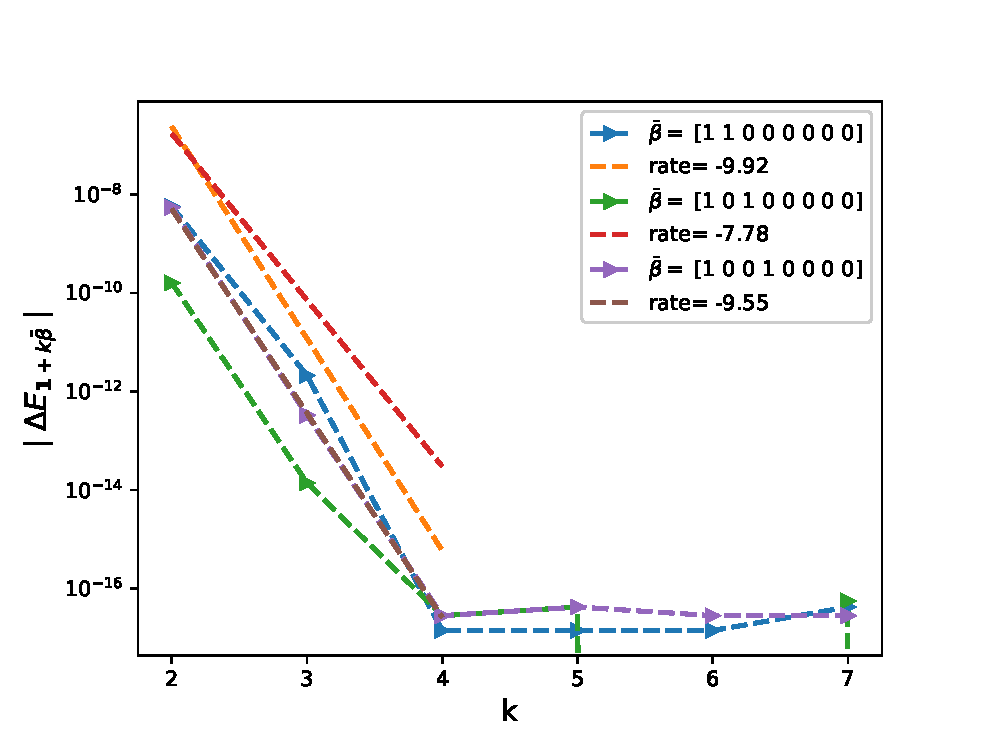
\includegraphics[width=1\linewidth]{./figures/rBergomi_mixed_error_rates/without_change_measure/N_4/H_002/mixed_difference_order2_rbergomi_4steps_H_002_K_1_totally_hierarch_with_rate_W1}
		\caption{}
		\label{fig:sub3}
	\end{subfigure}%
	\begin{subfigure}{.4\textwidth}
		\centering
		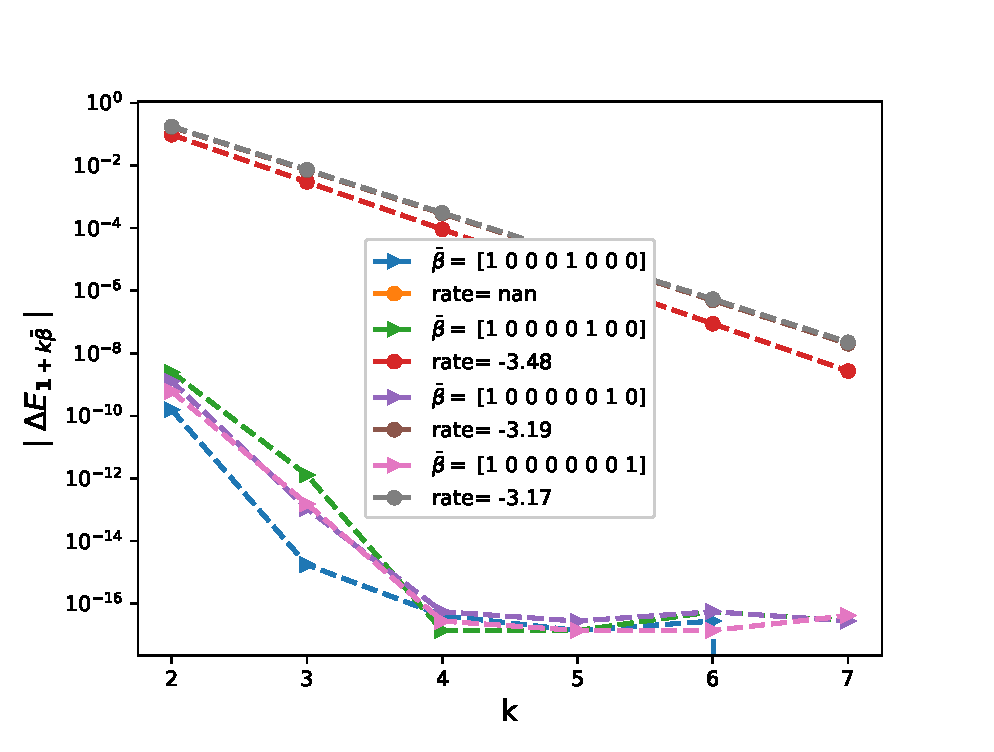
\includegraphics[width=1\linewidth]{./figures/rBergomi_mixed_error_rates/without_change_measure/N_4/H_002/mixed_difference_order2_rbergomi_4steps_H_002_K_1_totally_hierarch_with_rate_W2}
		\caption{}
		\label{fig:sub4}
	\end{subfigure}
	
	\caption{The rate of error convergence of  second order differences $\abs{\Delta \text{E}_{\boldsymbol{\beta}}}$, defined by \eqref{eq:Work_error_contributions},  ($\boldsymbol{\beta}=\mathbf{1}+k \bar{\boldsymbol{\beta}}$) with respect to $\mathbf{W}^{(1)}$ (a)  and  with respect to $\mathbf{W}^{(2)}$ (b), for parameter set $2$ in Table \ref{table:Reference solution, using MC with $500$ time steps, of Call option price under rBergomi model, for different parameter constellation.}. The number of quadrature points used in the $i$-th dimension is $N_i=2^{\beta_i-1}+1$.}
	\label{fig:second_diff_comp_K_1_H_002}
\end{figure}

\FloatBarrier

%
%\begin{remark}
%	In this paper, we limited ourselves to designing a novel alternative method  based on hierarchical adaptive sparse grids quadrature for computing option prices under the rBergomi model. Giving the significant performance gains of our novel designed algorithm, we expect that designing a method based on QMC can bring similar or more gains as  our approach.
%\end{remark}


%\subsubsection{MISC error estimate}
%
%
%In our case, once we fix $N$, we define from \eqref{BS_formula_rbergomi_2}
%
%\begin{equation*}
%F^N=C_{\text{BS}}(G(\mathbf{W}^{(1)},\mathbf{W}^{(2)})) \PERIOD
%\end{equation*}
%We introduce the set $C^0(\rset)$ of real-valued continuous functions over $\rset$, and the subspace of polynomials of degree at most $q$ over $\rset$, $\mathbb{P}^q(\rset) \subset C^0(\rset)$. Next,
%we consider a sequence of univariate Lagrangian interpolant operators in each dimension $Y_n$ ($1 \le n \le 2N$), that is, $\{U_n^{m(\beta_n)}\}_{\beta_n \in \nset_+}$ (we refer to the value $\beta_n$ as the interpolation level). Each interpolant is built over a set of $m(\beta_n)$ collocation points, $\mathcal{H}^{m(\beta_n)}=\{y^1_n,y^2_n,\dots,y^{m(\beta_n)}_n\} \subset \rset$, thus, the interpolant yields a polynomial approximation,
%\begin{equation*}
%U^{m(\beta_n)}:C^0(\rset) \rightarrow \mathbb{P}^{m(\beta_n)-1}(\rset), \quad U^{m(\beta_n)}[F^N](y_n)= \sum_{j=1}^{m(\beta_n)} \left( f(y^j_n) \prod_{k=1;k \neq j}^{m(\beta_n)} \frac{y_n-y_n^k}{y_n^j-y_n^k}\right) \PERIOD
%\end{equation*}
%The $2N$-variate Lagrangian interpolant can then be built by a tensorization of univariate interpolants: denote by $C^0(\rset^{2N})$ the space of real-valued $2N$-variate continuous functions over $\rset^{2N}$ and by $\mathbb{P}^{\mathbf{q}}(\rset^{2N}) = \otimes_{n=1}^{2N} \mathbb{P}^{\mathbf{q}_n}(\rset)$ the subspace of polynomials of degree at most $q_n$ over $\rset$, with $\mathbf{q}=(q_1,\dots,q_{2N})\in  \nset^{2N}$, and consider a multi-index $\boldsymbol{\beta} \in \nset^{2N}_+$ assigning the interpolation level in each direction, $y_n$, then  the multivariate interpolant can then be written as
%$$U^{m(\boldsymbol{\beta})}: C^0(\rset^{2N}) \rightarrow \mathbb{P}^{m(\boldsymbol{\beta})-1}(\rset^{2N}) ,\quad  U^{m(\boldsymbol{\beta})}[F^N](\mathbf{y})= \bigotimes_{n = 1}^{2N} U^{m(\beta_n)} [F^N](\mathbf{y}) \COMMA $$
%Given this construction, we can define the MISC interpolant  for approximating $F^N$, using a set of multi indices $\mathcal{I} \in \nset^{2N}$ as
%\begin{equation}
%I^{\mathcal{I}}[F^N]= \sum_{\boldsymbol{\beta} \in \mathcal{I}} \Delta U_N^{\boldsymbol{\beta}} \COMMA
%\end{equation}
%where 
%\begin{equation*}
%\Delta_i U_N^{\boldsymbol{\beta}} = \left\{ 
%\aligned 
% U_N^{\boldsymbol{\beta}} &- U_N^{\boldsymbol{\beta}'}  \text{, with } \boldsymbol{\beta}' =\boldsymbol{\beta} - e_i, \text{ if } \boldsymbol{\beta}_i>0 \\
% U_N^{\boldsymbol{\beta}} &, \quad  \text{ otherwise,}
%\endaligned
%\right.
%\end{equation*}
%where $e_i$ denotes the $i$th $2N$-dimensional unit vector. Then, $\Delta
%U_N^{\boldsymbol{\beta}}$ is defined as
%\begin{equation*}
%\Delta U_N^{\boldsymbol{\beta}} = \left( \prod_{i=1}^{2N} \Delta_i \right) U_N^{\boldsymbol{\beta}}.
%\end{equation*}
%We define the interpolation error induced by MISC as
%\begin{equation}
%e_{N}= F^N-I^{\mathcal{I}}[F^N] \PERIOD
%\end{equation}
%One can have a bound on the interpolation error of MISC, $e_{N}$, by tensorizing one dimensional error estimates, and  then simply integrate that bound to get the MISC quadrature error, $\mathcal{E}_Q(\text{TOL}_{\text{MISC}},N)$, defined in \eqref{eq:total_error}. However, we think that this will  not lead to a sharp error estimate for MISC. Another strategy for estimating the MISC quadrature error, is to estimate $\expt{e_N}$ using MC by sampling directly $e_N$. Finally,  one can learn the error curve as a way to reduce the extra burden that comes from estimating the MISC error.
%
%If we define $Y=F^N+(Q_N^{\mathcal{I}}-I^{\mathcal{I}}[F^N])$ (where $Q_N^{\mathcal{I}}$ is the MISC quadrature estimator, defined in \eqref{eq:MISC_quad_estimator}), then we have
%\begin{align}\label{eq:Control_variate}
%\expt{Y}&=\expt{F^N}\nonumber\\
%Var[Y]&=Var[e_N]< Var[\mathcal{A}_{\text{MC}}]\COMMA
%\end{align}
%where $\mathcal{A}_{\text{MC}}$ is the MC estimator for $\expt{F^N}$.
%
%\eqref{eq:Control_variate} shows that MISC can be seen as a control variate for MC estimator and consequently as a powerful variance reduction tool.
%
%\red{\textbf{Question $2$}: Do we just motivate this idea of variance reduction, or do we need also to provide more details here?
%}
%
%\red{\textbf{Question $3$}: What are the points that you suggest we give more details about in  this section?
%}

\subsection{Brownian bridge construction}\label{sec:Brwonian bridge construction}
In the literature of adaptive sparse grids and  QMC, several hierarchical path generation methods (PGMs) or transformation methods have been proposed to reduce the effective dimension. Among these transformations, we cite  the Brownian bridge (Bb)  construction \cite{morokoff1994quasi,moskowitz1996smoothness,caflisch1997valuation}, the principal component analysis (PCA)  \cite{acworth1998comparison} and the linear transformation (LT) \cite{imai2004minimizing}.

In our context, the Brownian motion on a time discretization  can be constructed either sequentially using a standard random walk construction, or hierarchically using   other PGMs as listed above. For our purposes, to make an effective use of MISC, which benefits from anisotropy, we use the Bb construction since it produces  dimensions with different importance for MISC, contrary to a random walk procedure for which all the dimensions of the stochastic space have equal importance. \red{In fact, Bb uses the first several coordinates of the low-discrepancy points to determine the general shape of the Brownian path, and the last few coordinates influence only the fine detail of the path. Consequently, this transformation  reduces the effective dimension  of the problem, which results in accelerating the MISC method by reducing the computational cost}.

Let us denote $\{t_i\}_{i=0}^{N}$ the grid of time steps. Then the Bb construction \cite{glasserman2004monte} consists of the following: given a past value $B_{t_i}$ and a future value $B_{t_k}$, the value $B_{t_j}$ (with $t_i < t_j < t_k$) can be generated according to 
\begin{equation*}
B_{t_j}=(1-\rho) B_{t_i}+\rho B_{t_k}+ \sqrt{\rho (1-\rho)(k-i) \Delta t} z, \: z \sim \mathcal{N}(0,1) \COMMA
\end{equation*}
where $\rho=\frac{j-i}{k-i}$.  


%In particular, if $N$ is a power of $2$, then given $B_0=0$, Bb generates the Brownian motion at times $T, T/2,T/4,3T/4,\dots$ according
%\begin{align}\label{eq:BB construction}
%	B_T&=\sqrt{T}z_1\nonumber\\
%	B_{T/2}&= \frac{1}{2}(B_{0}+B_{T})+\sqrt{T/4}z_2= \frac{\sqrt{T}}{2} z_1+\frac{\sqrt{T}}{2} z_2\nonumber\\
%	B_{T/4}&=\frac{1}{2} (B_{0}+B_{T/2})+\sqrt{T/8}z_3= \frac{\sqrt{T}}{4} z_1+\frac{\sqrt{T}}{4} z_2+\sqrt{T/8}z_3\nonumber\\
%	\vdots \nonumber\\
%\end{align}
%where $\{z_j\}_{j=1}^{N}$ are independent standard normal variables.  In Bb construction scheme given by \eqref{eq:BB construction}, the most important values that determine the large scale structure of Brownian motion are the first components of $\mathbf{z} = (z_1,\dots,z_N)$.



%\begin{remark}
%In this paper, we chose to couple Brownian bridge construction with the MISC solver to reduce the effective dimension, since it is the less costly option in terms of computational work and the easiest to implement. We did not investigate the performance of MISC when coupling it with other hierarchical path generations method such as PCA or LT, which could be left as a future work that looks for the optimal PGM to couple with MISC in this context.
%\end{remark}
%


\subsection{Richardson extrapolation}\label{sec:Richardson extrapolation}
Another transformation that we couple with MISC is Richardson extrapolation \cite{talay1990expansion}. In fact, applying level $K_\text{R}$ (level of extrapolation) of Richardson extrapolation  dramatically reduces the bias, and as a consequence reduces the  number of time steps $N$ needed in the coarsest level to achieve a certain error tolerance. As a consequence, Richardson extrapolation directly reduces  the total dimension of the integration problem for achieving some error tolerance.

\red{Let us denote by $(X_t)_{0 \le t \le T}$ a certain stochastic process and by $(\hat{X}_{t_i}^h)_{0 \le  t_i \le T}$ its approximation using a suitable  scheme with a time step $h$.  Then, for sufficiently small $h$, and a suitable smooth function $f$, we assume that}
\begin{align}\label{Euler_weak_error_strenghten}
	\expt{f(\hat{X}_T^h)}= \expt{f(X_T)} + c h +\Ordo{h^2} \PERIOD
\end{align}
Applying \eqref{Euler_weak_error_strenghten} with discretization step $2h$, we  obtain
\begin{align*}
	\expt{f(\hat{X}_T^{2h})}= \expt{f(X_T)} + 2 c h +\Ordo{h^2} \COMMA
\end{align*}
implying
\begin{align*}
	2 \expt{f(\hat{X}_T^{2h})}- \expt{f(\hat{X}_T^{h})} =\expt{f(X_T)} + \Ordo{h^2} \PERIOD
\end{align*}
For higher levels of extrapolations, we use the following: Let us denote by $h_J=h_0 2^{-J}$ the grid sizes (where $h_0$ is the coarsest grid size), by $K_\text{R}$ the level of the Richardson extrapolation, and by $I(J,K_\text{R})$ the approximation of $\expt{f((X_T)}$ by terms up to level $K_\text{R}$ (leading to a weak error of order $K_\text{R}$), then we have the following recursion 
\begin{align*}
I(J,K_\text{R})=\frac{2^{K_\text{R}}\left[I(J,K_\text{R}-1)-I(J-1,K_\text{R}-1)\right]}{2^{K_\text{R}}-1},\quad J=1,2,\dots, K_\text{R}=1,2,\dots
\end{align*}
\begin{remark}
We emphasize that throughout our work, we are interested in the pre-asymptotic regime (a small number of time steps), and the use of Richardson extrapolation is justified by our observed experimental results in that regime (see Section \ref{sec:Weak error plots_no_change}),  which suggest  a convergence of order one for the weak error. Although, we do not claim that the observed rates will scale well in the asymptotic regime, we did observe that the pre-asymptotic regime is enough to get sufficiently accurate estimates for the option prices. \red{We emphasize that, to the best of our knowledge, no proper weak error analysis has been done in the rough volatility context}. 
\end{remark}
